%************************************************
\chapter{Methodology}\label{ch:methodology}
%************************************************

The purpose of this chapter is to first formulate the research questions that we examine in our work
and then propose our method of answering them.

\section{Research Questions}\label{sec:research_questions}

In the \nameref{ch:example_chapter} chapter we dicussed the different meanings of structural and dataflow-based interactions.
With this knowledge, we can answer many interesting research topics. 
These topics include patterns in feature development and usage of commits therin as well as findings about how likely seemingly unrelated commits are to affect features inside a program.

\subsection*{\textbf{RQ1: How do commits and features structurally interact with each other?}}

We intend to research two main properties which already provide a lot of insight into the development process of features and best practices of commits therein.
Firstly, we examine the amount of commits features interact with structurally.
This gives us a direct estimate on how many commits were used in the development of a feature.
Our analysis also allows us to measure the size of feature, which can put the amount of commits used to implement a feature into perspective.
Secondly, we want to examine how many features a commit interacts with structurally, e.g. how many features a commit usually changes. 
This is especially interesting when considering best practices surrounding the usage of commits.
It is preferred to keep commits atomic\cite{hundhausen2021commit_metrics} meaning they should only deal with a single concern.
As different features implement separate functionalities, it's unlikely for a commit to change several features while dealing with the same concern.
Transferring this to our work, high quality commits should mostly change a single feature.
Acquiring data on this issue might show how strictly this policy is enforced in the development of features across different projects. 

\subsection*{\textbf{RQ2: How do commits interact with features through dataflow?}}

Investigating dataflow can unveil interactions between parts of a program that were previously hidden from programmers.
This can help a programmer understand the extent to which new changes affect other parts of a program.
Deploying the introduced analysis in a direct manner could even aid a programmer when fixing bugs of features.
Bugs occuring in certain features could be traced back to the authors responsible for them by factoring in recent commits affecting said features through dataflow. \\
Previous research has laid the groundwork for researching dataflow interactions between different parts of a program.
However, it has focused solely on dataflow interactions between commits.
That's why we aim to provide first insights on the properties of dataflow-based CFIs.
Specifically, we investigate how connected commits and features are by analyzing the amount of features a commit usually affects through dataflow.
Knowing what fraction of all commits contributing code to a project are part of dataflow-based interactions can show how often new commits affect the data of a feature. 
Regarding this, it is worth considering that commits constituting code of a feature are very likely to influence said feature through dataflow, as dicussed in section \ref{sec:combination_cfis}.
Since structural interactions coinciding with dataflow interactions are so obvious, programmers are also much more aware of them. 
Depending on the prevalence of feature regions in a project's code space, this could heavily skew the data in one direction, as a large portion of all dataflow interactions would stem from these obvious interactions. 
Therefore we want to especially focus on commits that aren't part of a feature, because programmers might not be aware or intend that changes introduced with these commits also affect features through dataflow. 
With the gathered information, another interesting aspect of dataflow-based CFIs to examine, is the relationship between the size of a feature and the number of outside commits interacting with it through dataflow.
Determining to what extent feature size is the driving factor in this, could tell us whether it is worth considering other possible properties of features responsible for the number of commits affecting its data.

\subsection*{\textbf{RQ3: How do authors interact with features?}}

Usually there are many programmers working on the same software project, implementing different features, sometimes alone, sometimes with the help of colleagues.
We want to shine some light on the exact statistics of this by combining structural commit-feature interactions with high-level repository information.
One major question we want to answer is how many authors implement a feature on average, where considering the size of a feature could help put this data into perspective.
The collected results could serve as advice for software companies on how to allocate programmers on to-be implemented features. 

\begin{center}
\begin{tabular}{cc}
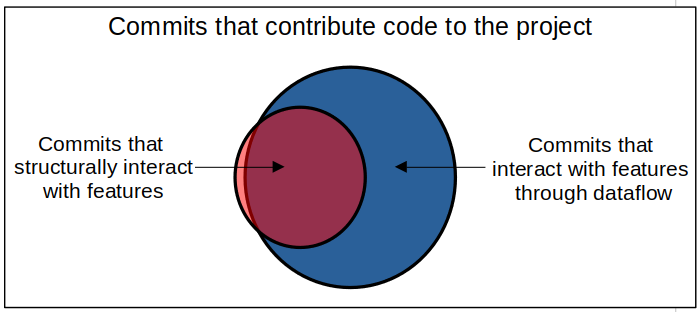
\includegraphics[height=6cm]{gfx/Commits-of-a-Software-Project.png}
\end{tabular}
\captionof{figure}{Kinds of commits in software projects investigated in this work. In the first two \textbf{RQs} we have discussed different kinds of commits and the ways in which they interact with features. 
Figure 1 showcases them in a venn diagram and illustrates the dependencies and divisions between them.}
\end{center}
